% 2013 四川卷文科第 12 题：平行四边形 ABCD，对角线 AC、BD 交于点 O。
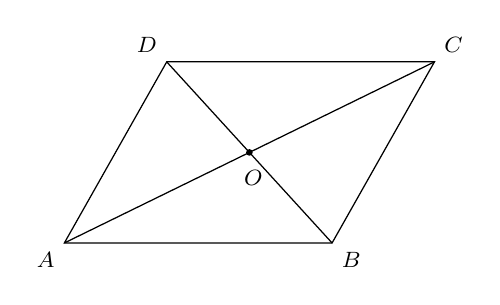
\begin{tikzpicture}[font=\footnotesize, line width=0.45pt, scale=1]
  \coordinate (A) at (0,0);
  \coordinate (B) at (3.4,0);
  \coordinate (C) at (4.7,2.3);
  \coordinate (D) at (1.3,2.3);
  \coordinate (O) at (2.35,1.15);
  \draw (A) -- (B) -- (C) -- (D) -- cycle;
  \draw (A) -- (C);
  \draw (B) -- (D);
  \fill (O) circle (1.2pt);
  \node[below left]  at (A) {$A$};
  \node[below right] at (B) {$B$};
  \node[above right] at (C) {$C$};
  \node[above left]  at (D) {$D$};
  \node[below]       at (2.40,1.05) {$O$};
\end{tikzpicture}
